\documentclass{article}

\usepackage[margin=0.5in]{geometry}
\usepackage{graphicx}
\usepackage{enumitem}
\usepackage{parskip}
\usepackage[usenames]{xcolor}
\usepackage{listings}
\usepackage{hyperref}
\usepackage{caption}
\usepackage{amsmath}
\usepackage{longtable}
\usepackage{booktabs}

\lstdefinelanguage{vns}
{keywords={add,sub,mul,div,and,orr,xor,nan,clz,cnt,lsr,lsl,abs,rnd,cmp,jiz,jnz,jgz,jlz,jge,jle,biz,bnz,bgz,blz,bge,ble,blx,ldr,str,pop,psh,
           who,wht,qcs,qct,qbp,qck,gnd,whr,dst,cvr,ded,sht,dir,wlk,crl,swm,cap,rtt,hid,say,rad,yel,ear,die,nrt,nre,est,soe,sot,sow,wst,nrw,
           wcs,wct,wbp,wcl,tcs,tct,tbp,tcl,pnt,ccs,cct,cbp,ccl,ucs,uct,ubp,ucl,dcs,dct,dbp,dcl,mcs,mct,mbp,mcl,rcs,rct,rbp,rcl,tim,dly,adv,
           ask,plz,beg,gvl,kmk,sac,bom,air,sum,hak,emp,all,rmt,rsn,res,ref,rms,rmf,rss,rsf,rrs,rrf,wmt,wsn,wes,wef,wms,wmf,wss,wsf,wrs,wrf,
           qhi,qrs,qsh,qpr,qsu,qmv,itf,fad,fsu,fmu,fdv,cel,rtf,sin,cos,tan,pow,asn,acs,atn,log,fcp,mle,set,css,cfs,wss,wfs,gup,sup,cam,unc,
           hip,nmr,ist,tgt,lie,mor,wir,cut,snd,dig,mlf,run,hit,raw},
 sensitive=false,
 comment=[l]{;},
}

\definecolor{grey}{rgb}{0,0.6,0}
\lstset{
    keywordstyle=\color{blue},
    commentstyle=\color{grey}
}


\newcommand{\vnscode}[1]{\colorbox{lightgray}{\lstinline[language=vns]{#1}}}

\newcommand{\UT}{\lower-0.5ex\hbox{u}\kern-1.1ex T}
\newcommand{\RT}{\lower-0.5ex\hbox{r}\kern-0.65ex T}
\newcommand{\RP}{R\kern-0.85ex P}

\title{Von Neumann Standing -- Instructions}
\date{\today}
\author{Louis A. Burke}

\begin{document}
\maketitle
\clearpage
\renewcommand{\baselinestretch}{0.9}\normalsize
\tableofcontents
\renewcommand{\baselinestretch}{1.0}\normalsize
\clearpage
\listoftables
\clearpage

\section{Introduction}

A game of Von Neumann Standing is played between two sets of programs. It
simulates a wartime battle over a river. The winner is whichever team captures
the enemy base.

\subsection{Units}

Each team consists of 11 units. Each unit runs its own program to determine its
actions. The team with the smartest programs will win the game.

The first unit is the captain. The captain isn't as effective in combat as the
rest of the team, but can defend itself. Its primary role is to requisition
additional resources and coordinate the movements of its team.

The second unit is the mortar. The mortar has to spend time setting up and
tearing down its weapon in order to fire it or move. While largely incapable of
defending itself, the mortar can drop area of effect shells on units from any
distance, ignoring cover.

The third unit is the sniper. The sniper can camouflage itself to make it
difficult for other units to see it. It can fire accurate bullets from afar and
through cover to dislodge the hardiest of units. You can be sure the sniper will
be a prime target for the enemy if spotted.

The fourth and fifth units are the engineers. They can construct defenses such
as cover and barbed wire. They are not the best in combat, but can tear through
enemy defenses with ease.

The sixth and seventh units are the machine gunners. Like the mortar they have
to setup and tear down their weapons in order to fire and move. Once setup
however, they can protect themselves well with the most powerful short-range
weapon in the game. It is unwise for any unit to approach a setup machine gun,
but mortars and snipers can sometimes take them on.

The eighth and ninth units are the scouts. They can move faster than any other
unit. While not very effective from afar, their shotgun will make short work of
nearby enemies. Additionally they can spot camouflaged snipers and have extra
visibility. The scouts can maintain constant communication with their sniper to
call in prospective targets.

The tenth and eleventh units are the riflemen. They are the primary soldiers of
the squad. Their relative expandability makes them the main offensive unit. They
can respond to support requests and offer tactical information to the rest of
the squad.

\subsection{Upgrades}

Each unit can upgrade its processor in order to execute its code faster. There
are four systems to be upgraded. The cache can be upgraded in both size and
algorithm. The branch predictor can be upgraded to make branches faster. Finally
the clock rate of the processor itself can be upgraded.

\subsection{Map}

The game is played on a 32 by 16 grid, with a team at either end. Separating the
teams is a large river. The river provides no cover, and nothing can be built on
it, nor setup on it. Both captains have the river marked for air strikes, so it
is unwise to leave any unit in it for long.

\clearpage

\section{Rules}

\subsection{Resources}

The game has only two resources. The first is the implicit resource of time. The
game operates on a universal clock cycle. One iteration of this cycle is
referred to as a \textit{Universal Tick} or \UT. However, each unit does not
execute an instruction every universal tick. Instead each of their
\textit{Relative Ticks} or \RT\ happen only on some of the universal ticks
(depending on CPU speed).

On top of time there is an explicit resource shared by each member of a team.
These are the team's \textit{Resource Points} or \RP. On each \UT\ each team
gains one \RP. \RP\ can be spent on upgrades and munitions.

\subsection{Upgrades}

\RP can be spent to upgrade the components of each unit's processor. Units can
also downgrade their components to return half of the resources they spent to
upgrade them.

\subsubsection{Cache Size}

The first system that can be upgraded is the cache size. By default each unit
has no cache whatsoever, however the cache can be upgraded up to 65536 entries.
The sizes and costs of the upgrades are summarized below.

\begin{minipage}{\textwidth}
\captionof{table}{Cache Size Upgrades}
\centering
\begin{tabular}{lll}
    \hline Level & \# Entries & Cost From Previous (\RP) \\ \hline
    0 & 0 & 0 \\
    1 & 64 & 32 \\
    2 & 1024 & 64 \\
    3 & 4096 & 256 \\
    4 & 65536 & 1024 \\
\end{tabular}
\end{minipage}

\subsubsection{Cache Type}

The second system that can be upgraded is the caching algorithm used by the
cache. By default each unit uses a 1-way set associative cache, however the
cache type can be upgraded up to a fully associative algorithm. The sizes and
costs of the upgrades are summarized below.

\begin{minipage}{\textwidth}
\captionof{table}{Cache Type Upgrades}
\centering
\begin{tabular}{lll}
    \hline Level & \# Algorithm & Cost From Previous (\RP) \\ \hline
    0 & One-way set associative & 0 \\
    1 & Two-way set associative & 32 \\
    2 & Four-way set associative & 64 \\
    3 & Eight-way set associative & 256 \\
    4 & Fully associative & 1024 \\
\end{tabular}
\end{minipage}

\subsubsection{Branch Predictor}

The third system that can be upgraded is the branch prediction algorithm. By
default no branch prediction is done and all branches take extra time, however
the branch predictor can be upgraded to a perfect oracle that always predicts
branches correctly. The algorithms and costs of the upgrades are summarized
below.

\begin{minipage}{\textwidth}
\captionof{table}{Branch Predictor Upgrades}
\centering
\begin{tabular}{lll}
    \hline Level & \# Algorithm & Cost From Previous (\RP) \\ \hline
    0 & Always Wrong & 0 \\
    1 & 1-bit saturation counter & 32 \\
    2 & 2-bit saturation counter & 64 \\
    3 & Two-level 2-bit saturation counter & 256 \\
    4 & Perfect prediction & 1024 \\
\end{tabular}
\end{minipage}

\subsubsection{CPU Speed}

The fourth system that can be upgraded is the CPU clock speed. By default one
\RT occurs every 8 \UT, however the clock speed can be upgraded to execute one
\RT every \UT. The speeds and costs of the upgrades are summarized below.

\begin{minipage}{\textwidth}
\captionof{table}{CPU Speed Upgrades}
\centering
\begin{tabular}{lll}
    \hline Level & \# \UT/\RT & Cost From Previous (\RP) \\ \hline
    0 & 8 & 0 \\
    1 & 6 & 64 \\
    2 & 4 & 128 \\
    3 & 2 & 512 \\
    4 & 1 & 2048 \\
\end{tabular}
\end{minipage}

\subsection{Shooting}

Each unit uses a different weapon. Different weapons take a different amount of
time to fire. The fire rate depends on the distance to the target, the cover the
target is behind, and the weapon being fired.

Each weapon has a base fire rate, a precision, and an accuracy.

The precision of a weapon applies to the distance of the shot, while the
accuracy applies to the cover that must be shot through. Cover directly in front
of the shooter does not count.
% Thought: maybe make units have to stand IN cover?

The exact formula for a weapon's firetime is:

$$t=b+pd+ac$$

Where $t$ is the time the shot takes in \RT, $p$ is the weapon's precision, $d$
is the distance to target, $a$ is the accuracy of the weapon, $c$ is the cover
between the shooter and the target.

The parameters of the weapons are:

\begin{minipage}{\textwidth}
\captionof{table}{Weapon Parameters}
\centering
\begin{tabular}{llllll}
    \hline
        Unit Name &
        Weapon Name &
        Base Rate ($b$) &
        Precision ($p$) &
        Accuracy ($a$) &
        Cost \\ \hline
    Captain & Pistol & 1 & 16 & 64 & 32 \RP \\
    Sniper & Sniper Rifle & 64 & 2 & 0 & 64 \RP \\
    Sniper & Hip Shot & 4 & 4 & 16 & 64 \RP \\
    Rifleman & Rifle & 4 & 4 & 16 & 64 \RP \\
    Engineer & Light Machinegun & 8 & 8 & 32 & 32 \RP \\
    Machinegunner & Machinegun & 1 & 8 & 64 & 64 \RP \\
    Scout & Shotgun & 8 & 16 & 4 & 64 \RP \\
    Mortar & Shell & 512 & 0 & 0 & 256 \RP \\
\end{tabular}
\end{minipage}

Additionally units can lie prone. A prone unit will not be hit by bullets that
pass overhead (only by those targeted directly at their coordinate), however
they will be hit by a mortar's shell and move at half their usual speed.

\subsection{Terrain}

There are six types of terrain in the game. The most common kind is open grass.
Open grass provides no cover but can be built upon by engineers. Wire is one of
the structures that can be built by engineers. It does not provide cover but
does impede unit movement. Cover can also be built by engineers. It doesn't
obstruct movement but does provide cover.

In the middle of the map is the river. Water tiles severely obstruct movement
and provide a sense of negative cover. Beach tiles similarly don't provide
cover, but movement is easy on them. Both water and beach tiles share a couple
properties. First nothing can be built on them, nor can units set up on them.
Additionally they do not count as increased distance for weapon shots, so a unit
on the shore can see all other units in or on the river as if they were right
next to them.

\subsection{Map}

The map is fixed and all coordinates are transformed relative to each team. As
such each team views the map's initial configuration as:

{\centering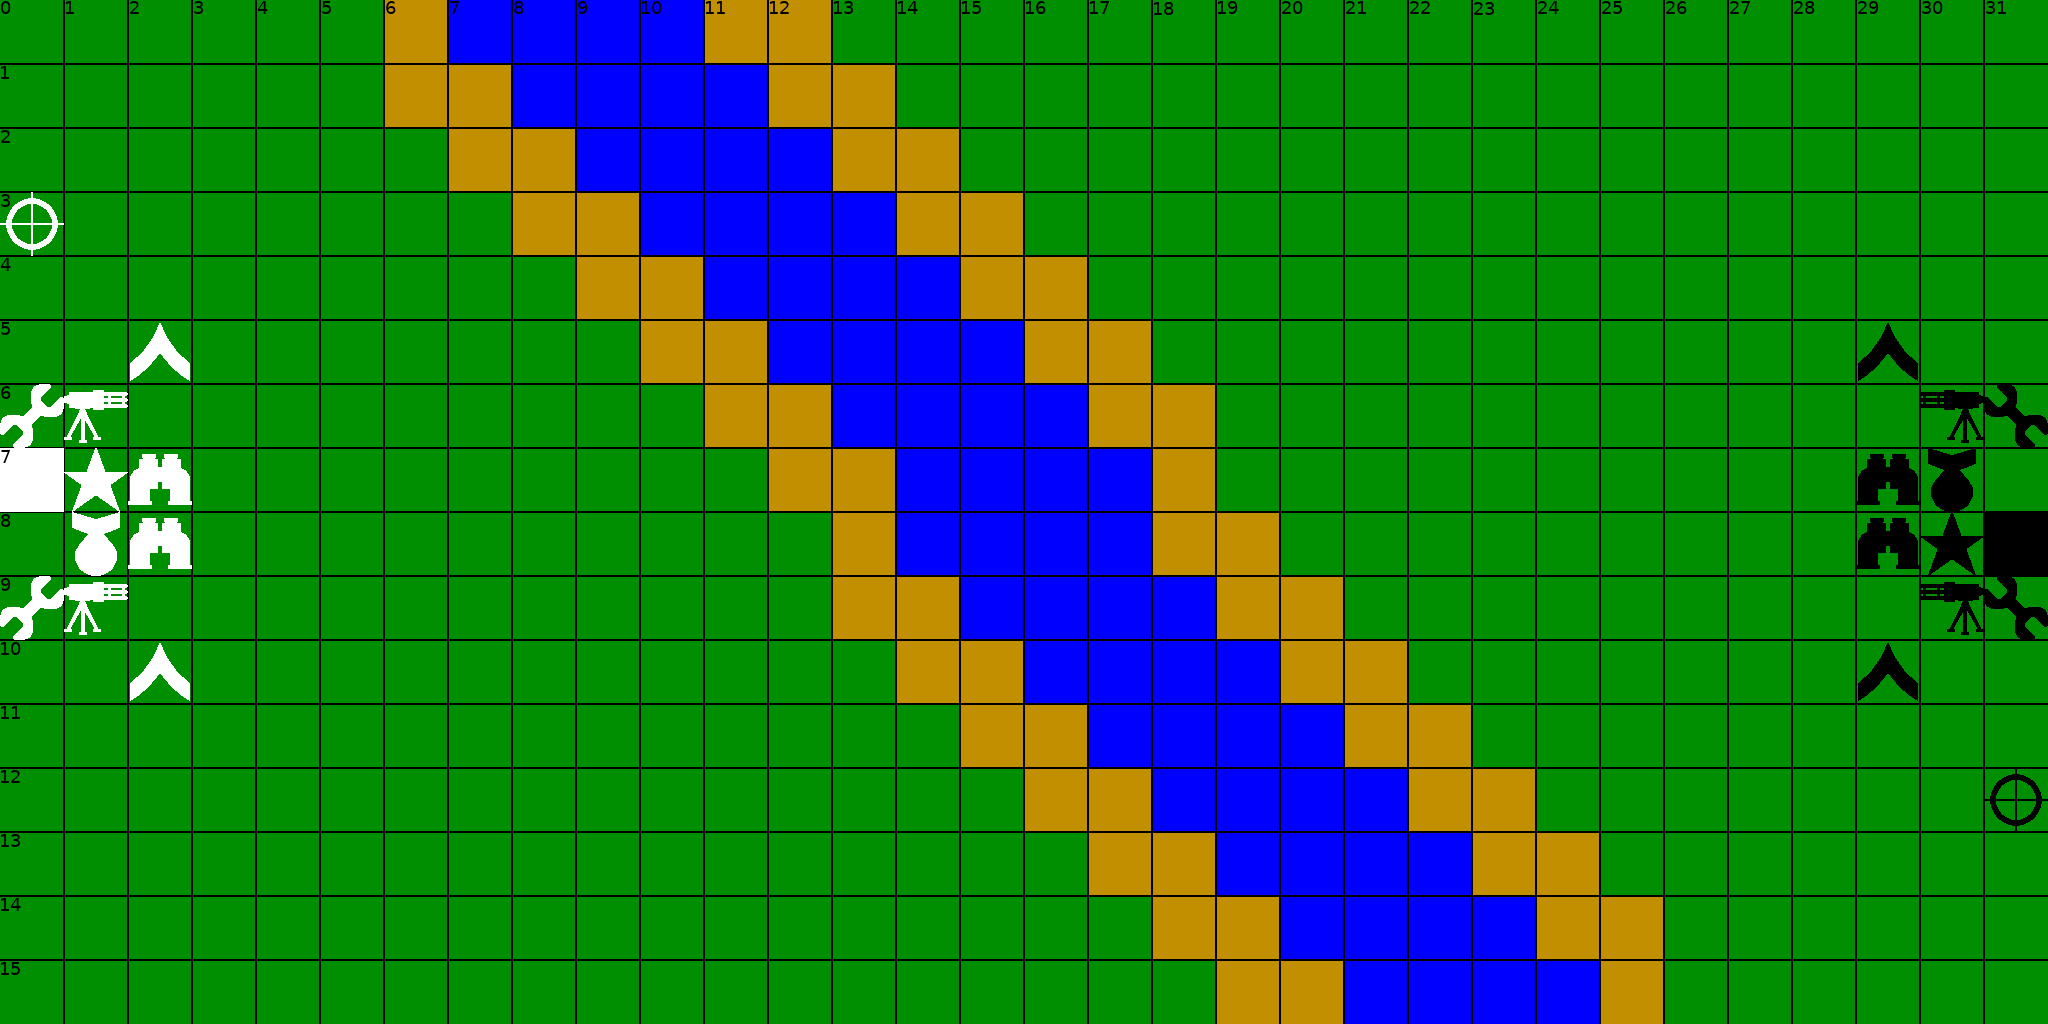
\includegraphics[width=\textwidth]{res/map.png}\par}

\subsection{Camouflage}

The sniper has the special ability to enter camouflage. This takes time and
while camouflaged the sniper's speed is halved. However, only scouts will be
able to see the sniper while it is camouflaged. When the sniper fires a shot it
automatically exits camouflage.

\subsection{Death}

When units die they stop execution entirely. Anything that examines them
directly will still find them in the state they were in before they were alive,
however indirect queries will not find them. For example they will never show up
as a nearest unit, but a dead captain will show up at the position it died at as
the captain's position.

\subsection{Victory}

A team wins when any unit captures the enemy's base. This takes a long time and
leaves the unit very vulnerable.

\section{Environment}

Each team's code runs it its own environment, with each unit running on their
own virtual machine. Each unit has 32 registers. The first 16 are the same for
each unit, while the second 16 are unit-specific. Additionally each unit has 1
megabyte of memory to run their code on.

\subsection{Command Layout}

The assembly language commands all take one of two forms.

The first form is the three-register command. For example \vnscode{add r1, r2,
r3} adds the values of registers 2 and 3 and stores the result in register 1.
These instructions leave 10 bits for a signed immediate value. This value is
accessible from register 12.  The assembler thus allows you to replace one
register with a 10-bit signed integer. This makes a common way to load a
register with a value to use \vnscode{add r1, r0, 10; Load 10 into r1}.

The second form is the single-register command. For example \vnscode{bnz r1,
123} will jump to address 123 if r1 is non-zero. These immediate values
typically refer to addresses, therefore it is common to use labels to refer to
them. These are any identifiers followed by a colon.

\subsection{Timing}

Different instructions take a different number of \RT to complete. Using
efficient instructions can get your units to react faster.

\subsection{Specifics}

This section indicates some of the specifics of the game. Things such as integer
representations of concepts and formal definitions of terms are described.

\subsubsection{Directions}

This table indicates the codes for each direction. North is always towards
decreasing Y values and East is always towards increasing X values (relative to
your team's coordinate system).

\begin{minipage}{\textwidth}
\captionof{table}{Direction Codes}
\centering
\begin{tabular}{lll}
    North-West (8) & North (1) & North-East (2) \\
    West (7) & & East (3) \\
    South-West (6) & South (5) & South-East (4) \\
\end{tabular}
\end{minipage}

\subsubsection{Terrains}

This table indicates the codes for each terrain type.

\begin{minipage}{\textwidth}
\captionof{table}{Terrain Codes}
\centering
\begin{tabular}{llllll}
    Grass & Wire & Cover & Beach & Water & Base \\ \hline
    1 & 2 & 3 & 4 & 5 & 6
\end{tabular}
\end{minipage}

\subsubsection{Units}

This table indicates the codes for each unit type. Different codes refer to
different team's units.

\begin{minipage}{\textwidth}
\captionof{table}{Unit Codes}
\centering
\begin{tabular}{lll}
    \hline Unit & Friendly ID & Enemy ID \\ \hline
    Captain & 1 & -1 \\
    Mortar & 2 & -2 \\
    Sniper & 3 & -3 \\
    Engineer (SS) & 4 & -4 \\
    Engineer (FS) & 5 & -5 \\
    Machinegunner (SS) & 6 & -6 \\
    Machinegunner (FS) & 7 & -7 \\
    Scout (SS) & 8 & -8 \\
    Scout (FS) & 9 & -9 \\
    Rifleman (SS) & 10 & -10 \\
    Rifleman (FS) & 11 & -11 \\
\end{tabular}
\end{minipage}

\subsubsection{Nearest}

The term nearest is used often in the game. Given the nature of the coordinate
system it is not clear what exactly the term implies.

In the game whenever a nearest computation is made a spiraling search pattern is
performed around the target square. This pattern can be visualized as:

{\centering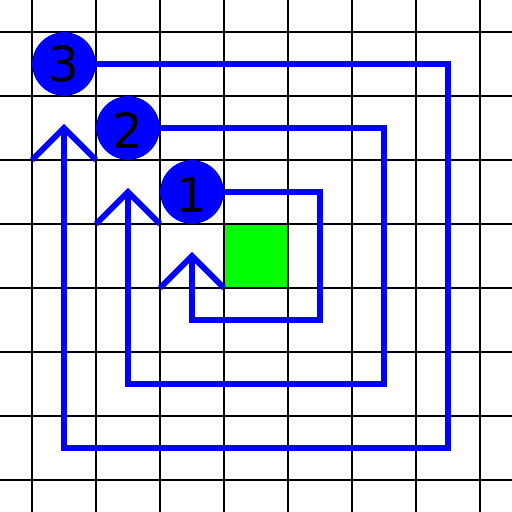
\includegraphics[width=0.5\textwidth]{res/nearest.png}\par}

This pattern is extended outwards indefinitely to cover the entire map aside
from the search square itself.

\subsubsection{Upgrade Levels}

Each upgrade level starts at 0 and is incremented by 1 when upgraded.

\subsection{Operations}

This section outlines all of the operations in the game. They are categorized
based on type.

\subsubsection{Arithmetic Operations}

The assembly language used in this game contains many of the typical
arithmetic instructions one might see in a traditional assembly language. These
instructions are summarized below.

\begin{minipage}{\textwidth}
\captionof{table}{Arithmetic Operations}
\label{table:arithmetic}
\centering
\begin{tabular}{llll}
    \hline \vnscode{CODE} & Instruction Name & Description & Time (\RT) \\ \hline
    \vnscode{ADD a, b, c} & Add & Adds b and c, storing the result in a. & 1 \\
    \vnscode{SUB a, b, c} & Subtract & Subtracts c from b, storing the result in a. & 1 \\
    \vnscode{MUL a, b, c} & Multiply & Multiplies b and c, storing the result in a. & 4 \\
    \vnscode{DIV a, b, c} & Divide & Divides b by c, storing the result in a. & 8 \\
    \vnscode{AND a, b, c} & Bitwise AND & Performs bitwise AND on b and c, storing the result in a. & 1 \\
    \vnscode{ORR a, b, c} & Bitwise OR & Performs bitwise OR on b and c, storing the result in a. & 1 \\
    \vnscode{XOR a, b, c} & Bitwise XOR & Performs bitwise XOR on b and c, storing the result in a. & 1 \\
    \vnscode{NAN a, b, c} & Bitwise NAND & Performs bitwise NAND on b and c, storing the result in a. & 1 \\
    \vnscode{CLZ a, b, c} & Count Leading Zeroes & Sets b to the number of leading zeroes in a, c to leading ones. & 1 \\
    \vnscode{CNT a, b, c} & Count & Sets b to the number of zeroes in a, c to the number of ones. & 1 \\
    \vnscode{LSR a, b, c} & Logical Shift Right & Shifts b right by c bits, storing the result in a. & 1 \\
    \vnscode{LSL a, b, c} & Logical Shift Left & Shifts b left by c bits, storing the result in a. & 1 \\
    \vnscode{ABS a, b, c} & Absolute Value & Stores the absolute value of a in b and its negative in c. & 1 \\
    \vnscode{RND a, b, c} & Random & Sets all 3 registers to random values. & 1 \\
\end{tabular}
\end{minipage}

\subsubsection{Branch Operations}

There are two kinds of branch instructions. They differ in how the branch
predictor works on them. Jump instructions are always assumed to be taken,
meanwhile branches make full use of the branch predictor. The exception is the
special unconditional branch and link instruction, which never fails. That
instruction saves the next address to be executed in register 14, the link
register -- this can be used to make subroutine calls. All branches take 1 \RT
to complete when they are correctly predicted, otherwise they take 8 \RT.

In order to efficiently branch based on values in registers a comparison
instruction is provided. It compares b and c and puts the normalized result in
a. Thus the value of the a register after execution will always be $1$, $-1$, or
$0$. The exact computation of the compare instruction is:

\begin{displaymath}
    a = \begin{cases}
        1 & \mbox{if } b > c \\
        -1 & \mbox{if } b < c \\
        0 & \mbox{if } b = c \end{cases}
\end{displaymath}

The branch instructions and comparison instruction are summarized below.

\begin{minipage}{\textwidth}
\captionof{table}{Branch Operations}
\label{table:branch}
\centering
\begin{tabular}{lll}
    \hline \vnscode{CODE} & Instruction Names & Descriptions \\ \hline
    \vnscode{CMP a, b, c} & Compare. & Compare b and c, storing the result in a. \\
    \vnscode{JIZ/BIZ a, i} & Jump/Branch zero. & If a is zero, go to i. \\
    \vnscode{JNZ/BNZ a, i} & Jump/Branch non-zero. & If a is not zero, go to i. \\
    \vnscode{JGZ/BGZ a, i} & Jump/Branch greater zero. & If a is greater than zero, go to i. \\
    \vnscode{JLZ/BLZ a, i} & Jump/Branch less zero. & If a is less than zero, go to i. \\
    \vnscode{JGE/BGE a, i} & Jump/Branch greater equal zero. & If a is not less than zero, go to i. \\
    \vnscode{JLE/BLE a, i} & Jump/Branch less equal zero. & If a is not greater than zero, go to i. \\
    \vnscode{BLX a, i} & Branch and Link. & Jump to a+i, set lr to next pc. \\
\end{tabular}
\end{minipage}

\subsubsection{Memory Operations}

There are four memory operations. Two of them are general-purpose while two of
them are designed for stack-based operation. Like branches their runtime is
dependent on the upgrade levels of the unit. In particular each unit has its own
cache. When a cell of memory is present in the cache then memory operations take
only one \RT, however when a cache miss occurs they take 8 \RT.

The stack based operations implicitly use register 13, the stack pointer. They
read and write to the address in said register after subtracting the immediate
value. Popping increments the register before reading while pushing decrements
it after writing. The immediate offset can be used to simulate multiple stacks
by using different offsets.

The memory instructions are summarized below.

\begin{minipage}{\textwidth}
\captionof{table}{Memory Operations}
\label{table:memory}
\centering
\begin{tabular}{lll}
    \hline \vnscode{CODE} & Instruction Names & Descriptions \\ \hline
    \vnscode{LDR a, b, c} & Load Register & Load the value in memory at location $b+c$ into a. \\
    \vnscode{STR a, b, c} & Store Register & Store the value in a into memory at location $b+c$. \\
    \vnscode{POP a, i} & Pop & Pops the top of the stack at memory location i into a. \\
    \vnscode{PSH a, i} & Push & Pushes a onto the top of the stack at memory location i. \\
\end{tabular}
\end{minipage}

\subsubsection{Float Operations}

Most units have access to a floating point arithmetic processor. These operate
on 32-bit floating point numbers using the same registers as other commands. In
general floating point operations are slower than their integer counterparts.
The exact format of the floating point processor is not specified, so it is only
safe to use the integer to float conversion to set floating point values.
Floating point trigonometric operations take place in radians.

Only the captain lacks a floating point processor.

The floating point instructions are summarized below.

\begin{minipage}{\textwidth}
\captionof{table}{Float Operations}
\label{table:float}
\centering
\begin{tabular}{llll}
    \hline \vnscode{CODE} & Instruction Names & Descriptions & Time (\RT) \\ \hline
    \vnscode{ITF a, i} & Integer to Float & Set a to floating point approximation of i. & 8 \\
    \vnscode{FAD a, b, c} & Float Add & Set a to floating point addition of b and c. & 8 \\
    \vnscode{FSU a, b, c} & Float Subtract & Set a to floating point subtraction of c from b. & 8 \\
    \vnscode{FMU a, b, c} & Float Multiply & Set a to floating point multiplication of b and c. & 32 \\
    \vnscode{FDV a, b, c} & Float Divide & Set a to floating point division of b by c. & 64 \\
    \vnscode{CEL a, b, c} & Ceiling & Set b to integer ceiling of a, c to integer floor. & 8 \\
    \vnscode{RTF a, i} & Register to Float & Set a to floating point approximation of a / i. & 8 \\
    \vnscode{SIN a} & Sine & Set a to floating point sine of a. & 64 \\
    \vnscode{COS a} & Cosine & Set a to floating point cosine of a. & 64 \\
    \vnscode{TAN a} & Tangent & Set a to floating point tanget of a. & 64 \\
    \vnscode{POW a, b, c} & Power & Set a to floating point power of b to c. & 64 \\
    \vnscode{ASN a} & Arcsine & Set a to floating point arcsine of a. & 64 \\
    \vnscode{ACS a} & Arccosine & Set a to floating point arccosine of a. & 64 \\
    \vnscode{ATN a} & Arctangent & Set a to floating point arctangent of a. & 64 \\
    \vnscode{LOG a, b, c} & Logarithm & Set a to the floating point base c logarithm of b. & 64 \\
    \vnscode{FCP a, b, c} & Float compare & Set a to the floating point comparison of b and c. & 8 \\
\end{tabular}
\end{minipage}

\subsubsection{Time Operations}

There are 3 time based operations. The first computes the current in-game time.
It provides time in \UT, \RT and as a sum of all \RT performed by your team. The
second and third allow units to offset their processors by 1 \UT.

The time instructions are summarized below.

\begin{minipage}{\textwidth}
\captionof{table}{Time Operations}
\label{table:time}
\centering
\begin{tabular}{llll}
    \hline \vnscode{CODE} & Instruction Names & Descriptions & Time (\RT) \\ \hline
    \vnscode{TIM a, b, c} & Time & Set a to \UT, b to \RT and c to \RT of team.  & 1 \\
    \vnscode{DLY} & Delay & Wait 1 \UT. & 1 \\
    \vnscode{ADV} & Advance & Next operation takes 1 less \UT. & 4 \\
\end{tabular}
\end{minipage}

\subsubsection{Query Operations}

There are many instructions that query the field of combat by coordinate to
ascertain information about the state of the game. All query operations
query a location defined by the x-coordinate in b and the y-coordinate in c.
The special query operation \vnscode{WHR} instead stores the query into b and c.

The query instructions are summarized below.

\begin{minipage}{\textwidth}
\captionof{table}{Query Operations}
\label{table:query}
\centering
\begin{tabular}{llll}
    \hline \vnscode{CODE} & Instruction Names & Descriptions & Time (\RT) \\ \hline
    \vnscode{WHO a, b, c} & Who & Set a to $0$ if no unit, $1$ if friendly unit, $-1$ if enemy unit. & 1 \\
    \vnscode{WHT a, b, c} & What & Set a to $0$ if no unit, or the unit code. & 1 \\
    \vnscode{QCS a, b, c} & Query Cache Size & Set a to $-1$ if no unit, or the unit's cache size upgrade level. & 1 \\
    \vnscode{QCT a, b, c} & Query Cache Type & Set a to $-1$ if no unit, or the unit's cache type upgrade level. & 1 \\
    \vnscode{QBP a, b, c} & Query Branch Predictor & Set a to $-1$ if no unit, or the unit's predictor upgrade level. & 1 \\
    \vnscode{QCK a, b, c} & Query Clock & Set a to $-1$ if no unit, or the unit's clock upgrade level. & 1 \\
    \vnscode{GND a, b, c} & Ground & Set a to the terrain type. & 1 \\
    \vnscode{DST a, b, c} & Distance & Set a to the distance from the location. & 4 \\
    \vnscode{CVR a, b, c} & Cover & Set a to the cover between us and the location. & 8 \\
    \vnscode{DIR a, b, c} & Direction & Set a to the direction towards the location. & 1 \\
    \vnscode{WHR a, b, c} & Where & Set b and c to the location of unit a, or $-1,-1$ if a is not visible. & 1 \\
\end{tabular}
\end{minipage}

\subsubsection{Search Operations}

There are 8 operations for searching for the nearest unit in a given direction.
Each of these operations returns the unit ID in a and its position in b and c.
If no unit is found it does not modify the registers. The search will only find
units directly due in those directions. All search operations take 4 \RT.

The search instructions are summarized below.

\begin{minipage}{\textwidth}
\captionof{table}{Search Operations}
\label{table:search}
\centering
\begin{tabular}{ll}
    \hline \vnscode{CODE} & Instruction Names \\ \hline
    \vnscode{NRT a, b, c} & Search North \\
    \vnscode{NRE a, b, c} & Search North-East \\
    \vnscode{EST a, b, c} & Search East \\
    \vnscode{SOE a, b, c} & Search South-East \\
    \vnscode{SOT a, b, c} & Search South \\
    \vnscode{SOW a, b, c} & Search South-West \\
    \vnscode{WST a, b, c} & Search West \\
    \vnscode{NRW a, b, c} & Search North-West \\
\end{tabular}
\end{minipage}

\subsubsection{Movement Operations}

There are 6 movement operations. The most common is the walk instruction which
merely moves you in a given direction. However units cannot walk through wire or
water. In order to move onto a water terrain a unit has to swim and in order to
move onto a wire terrain a unit has to crawl.

Scouts have the unique run command which acts exactly like move except that it
is much faster. Other units can only move faster by being summoned or
retreating.

Captains can summon units to themselves. The summoned unit will effectively
execute a run operation towards the captain until such time as they are adjacent
to him. This effectively pauses the unit's execution.

Similarly any unit can retreat. This causes them to similarly run towards their
team's base.

Be warned, summoning or retreating a unit that cannot move (such as one that is
boxed in or setup) may be unwise as they will no longer be able to execute
commands until they arrive at their destination.

When a unit's speed is halved all of the movement operations take twice as long.
In the case of snipers this can stack to up to a four fold increase. A unit
which is setup cannot move under any circumstances.

The movement instructions are summarized below.

\begin{minipage}{\textwidth}
\captionof{table}{Movement Operations}
\label{table:movement}
\centering
\begin{tabular}{lllll}
    \hline \vnscode{CODE} & Instruction Names & Descriptions & Time (\RT) & Units \\ \hline
    \vnscode{WLK a, b, c} & Walk & Walk in direction a, save resulting position in b and c. & 8 & All \\
    \vnscode{CRL a, b, c} & Crawl & Crawl in direction a, save resulting position in b and c. & 64 & All \\
    \vnscode{SWM a, b, c} & Swim & Swim in direction a, save resulting position in b and c. & 64 & All \\
    \vnscode{RTT} & Retreat & Begin retreating. No effect on registers. & ? & All \\
    \vnscode{SUM a} & Summon & Summons unit a. b and c ignored. & 8 & Captain \\
    \vnscode{RUN a, b, c} & Run & Run in direction a, save resulting position in b and c. & 1 & Scout \\
\end{tabular}
\end{minipage}

\subsubsection{Combat Operations}

There are a lot of combat instructions. The most common is the shoot instruction
which fires a bullet at the coordinate specified by b and c. If a shot kills a
unit then the a register is set to 1, otherwise it is set to 0. The time of the
shoot instruction has already been described based on the weapon parameters.

The sniper has a special hip shot instruction in which their weapon acts as if
it is a rifle rather than a sniper rifle.

The hide instruction makes a unit invisible (though not invulnerable) for a
duration. Execution is paused for that entire execution.

The capture instruction is used to win the game. Normally it is merely a 0-\RT\
no-op, but if the unit is on the enemy base it will win the game after 256 \RT!

Units can kill themselves with the die instruction. However, when compiled for
debugging the die instruction will instead log the values of the registers
passed to it.

The captain has two instructions that kill all of the units in the river or on
the beach. These take a long time and a lot of resources but can be very
effective at preventing the enemy from attacking. The bomb instruction costs 128
\RP and kills any unit in the river while the air strike instruction costs 64
\RP and kills any unit on the beach.

Mortars and machinegunners can do a melee attack around them to kill any unit
that gets too close. Machinegunners can even do a targeted melee attack that
is remarkably fast. Melee attacks do not cost any resources. The scout also has
a melee attack that is faster than shooting point-blank and is free.

Engineers can build and destroy defensive structures. Sand bags provide cover
while barbed wire impairs movement.

Most units also have the lie down and get up commands which make them lie prone
and stop lying prone respectively. Mortars and machinegunners instead have setup
and get up commands to change the setup state of their weapons.

Finally any unit can query the liveness of a unit type with the dead command. It
sets registers to 1 if the given unit is dead and 0 if they are alive.

The combat instructions are summarized below.

\begin{minipage}{\textwidth}
\captionof{table}{Combat Operations}
\label{table:combat}
\centering
\begin{tabular}{lllll}
    \hline \vnscode{CODE} & Instruction Names & Descriptions & Time (\RT) & Units \\ \hline
    \vnscode{SHT a, b, c} & Shoot & Shoot at b,c. Set a to 1 if hit or 0 otherwise. & ? & All \\
    \vnscode{HIP a, b, c} & Hip Shot & Shoot at b,c as rifleman. Set a as above. & ? & Sniper \\
    \vnscode{HID a, i} & Hide & Hide the unit for the duration & a+i & All \\
    \vnscode{CAP} & Capture & Try to capture the enemy base & 0/256 & All \\
    \vnscode{DIE a, b, c} & Die & Log arguments or die. & 0 & All \\
    \vnscode{BOM} & Bomb & Bomb the river. Arguments ignored. & 256 & Captain \\
    \vnscode{AIR} & Air Raid & Bomb the nearest beach. Arguments ignored. & 128 & Captain \\
    \vnscode{MLE} & Melee & Kill all units adjacent to this unit. & 16 & Mortar/MG \\
    \vnscode{MLF a} & Melee Forward & Melee in direction a. & 4 & MG \\
    \vnscode{HIT a} & Hit & Melee in direction a. & 16 & Scout \\
    \vnscode{WIR a, b, c} & Wire & Wire in direction a. Set b,c to total wire,cover count. & 8 & Engineer \\
    \vnscode{CUT a, b, c} & Cut Wire & Remove wire in direction a. Set b,c as above. & 8 & Engineer \\
    \vnscode{SND a, b, c} & Sandbag & Make cover in direction a. Set b,c as above. & 8 & Engineer \\
    \vnscode{DIG a, b, c} & Dig & Remove cover in direction a. Set b,c as above. & 8 & Engineer \\
    \vnscode{LIE} & Lie down & Set prone. & 64 & not Captain/Mortar/MG \\
    \vnscode{GUP} & Get up & Set not prone. & 64 & not Captain/Mortar/MG \\
    \vnscode{SET} & Set up & Set up weapon. & 128 & Mortar/MG \\
    \vnscode{GUP} & Get up & Tear down weapon. & 128 & Mortar/MG \\
    \vnscode{DED a, b, c} & Dead & Set b and c if unit $a$ or $-a$ is dead respectively. & 1 & All \\
    \vnscode{QHI a, b, c} & Query Hidden & Same as \vnscode{DED} but if hidden. & 1 & Mortar/Rifle \\
    \vnscode{QRS a, b, c} & Query Retreat/Summon & Same as \vnscode{DED} but if retreating or summoned. & 1 & Mortar/Rifle \\
    \vnscode{QSH a, b, c} & Query Shooting & Same as \vnscode{DED} but if shooting. & 1 & Mortar/MG/Scout/Rifle \\
    \vnscode{QPR a, b, c} & Query Prone & Same as \vnscode{DED} but if prone. & 1 & Mortar/MG/Scout/Rifle \\
    \vnscode{QSU a, b, c} & Query Setup & Same as \vnscode{DED} but if setup. & 1 & Mortar/Engineer/MG/Scout/Rifle \\
    \vnscode{QMV a, b, c} & Query Moving & Same as \vnscode{DED} but if moving. & 1 & Mortar/Engineer/MG/Scout/Rifle \\
\end{tabular}
\end{minipage}

\subsubsection{Communication Operations}

Each unit has two forms of communication with its team. The first is the open
communication to the entire team as a whole. The second is direct communication
to the team's captain. Each unit has its own communication channel with its
captain. Even the captain can leave himself personal messages on his
communication channel. Both communication systems are implemented as an
additional memory space equal to the size of memory.

Additionally specific direct forms of communication exist between certain units.

The communication instructions are summarized below.

\begin{minipage}{\textwidth}
\captionof{table}{Communication Operations}
\label{table:communication}
\centering
\begin{tabular}{lllll}
    \hline \vnscode{CODE} & Instruction Names & Descriptions & Time (\RT) & Units \\ \hline
    \vnscode{SAY a, i} & Say & Set captain's message i to a. & 8 & All \\
    \vnscode{RAD a, i} & Radio & Set a to captain's message i. & 8 & All \\
    \vnscode{YEL a, i} & Yell & Set team message i to a. & 16 & All \\
    \vnscode{EAR a, i} & Ear & Set a to team message i. & 16 & All \\
    \vnscode{HAK a, i} & Hack & Set enemy team message i to a. & 16 & Captain \\
    \vnscode{EMP a} & EMP & Set all enemy team messages to a. & 256 & Captain \\
    \vnscode{ALL a, i} & All & Set all team captain messages i to a. & 1 & Captain \\
    \vnscode{RMT a, i} & Read Mortar & Set a to mortar message i. & 1 & Captain \\
    \vnscode{RSN a, i} & Read Sniper & Set a to sniper message i. & 1 & Captain \\
    \vnscode{RES a, i} & Read Sniperside Engineer & Set a to sniperside engineer message i. & 1 & Captain \\
    \vnscode{REF a, i} & Read Farside Engineer & Set a to farside engineer message i. & 1 & Captain \\
    \vnscode{RMS a, i} & Read Sniperside MG & Set a to sniperside MG message i. & 1 & Captain \\
    \vnscode{RMF a, i} & Read Farside MG & Set a to farside MG message i. & 1 & Captain \\
    \vnscode{RSS a, i} & Read Sniperside Scout & Set a to sniperside scout message i. & 1 & Captain \\
    \vnscode{RSF a, i} & Read Farside Scout & Set a to farside scout message i. & 1 & Captain \\
    \vnscode{RRS a, i} & Read Sniperside Rifleman & Set a to sniperside rifleman message i. & 1 & Captain \\
    \vnscode{RRF a, i} & Read Farside Rifleman & Set a to farside rifleman message i. & 1 & Captain \\
    \vnscode{WMT a, i} & Write Mortar & Set mortar message i to a. & 1 & Captain \\
    \vnscode{WSN a, i} & Write Sniper & Set sniper message i to a. & 1 & Captain \\
    \vnscode{WES a, i} & Write Sniperside Engineer & Set sniperside engineer message i to a. & 1 & Captain \\
    \vnscode{WEF a, i} & Write Farside Engineer & Set farside engineer message i to a. & 1 & Captain \\
    \vnscode{WMS a, i} & Write Sniperside MG & Set sniperside MG message i to a. & 1 & Captain \\
    \vnscode{WMF a, i} & Write Farside MG & Set farside MG message i to a. & 1 & Captain \\
    \vnscode{WSS a, i} & Write Sniperside Scout & Set sniperside scout message i to a. & 1 & Captain \\
    \vnscode{WSF a, i} & Write Farside Scout & Set farside scout message i to a. & 1 & Captain \\
    \vnscode{WRS a, i} & Write Sniperside Rifleman & Set sniperside rifleman message i to a. & 1 & Captain \\
    \vnscode{WRF a, i} & Write Farside Rifleman & Set farside rifleman message i to a. & 1 & Captain \\
\end{tabular}
\end{minipage}


\subsubsection{Request Operations}

Many units have request instructions to ask other units to do things. These
often directly modify special registers on those units' processors. All request
instructions take 8\RT to complete. Once complete all of these instructions set
a to 1 if the target unit was alive or 0 if it wasn't.

Four of the request instructions are to ask the engineers to build cover and
wire at specific locations.

Two are to ask the captain to use his special river-based attacks. These
increment a special captain register by the immediate amount. This can be used
to ask with different amounts of forcefulness.

One is to ask the mortar to fire a shell at a specific location.

One is to ask riflemen for support. All riflemen will be able to see the latest
support request from both teams.

The request instructions are summarized below.

\begin{minipage}{\textwidth}
\captionof{table}{Request Operations}
\label{table:request}
\centering
\begin{tabular}{llll}
    \hline \vnscode{CODE} & Instruction Names & Descriptions & Units \\ \hline
    \vnscode{CSS a, b, c} & Cover Sniperside & Ask sniperside engineer for cover at b, c. & not Captain \\
    \vnscode{CFS a, b, c} & Cover Farside & Ask farside engineer for cover at b, c. & not Captain \\
    \vnscode{WSS a, b, c} & Wire Sniperside & Ask sniperside engineer for wire at b, c. & not Captain \\
    \vnscode{WFS a, b, c} & Wire Farside & Ask farside engineer for wire at b, c. & not Captain \\
    \vnscode{BOM a, i} & Bomb & Ask captain to bomb i times. & not Captain \\
    \vnscode{AIR a, i} & Air & Ask captain to air raid i times. & not Captain \\
    \vnscode{MOR a, b, c} & Mortar & Ask mortar to shoot b, c. & not Captain/Mortar \\
    \vnscode{SUP} & Support & Ask riflemen for support at b, c. & not Captain \\
\end{tabular}
\end{minipage}

\subsubsection{Resource Operations} % AKA Captain Specific

The resource instructions interact with the resource points of a team. Any unit
can query how many resources they have, but the captain can spend time
generating extra resources for the team. The captain can even try to sacrifice
units for more resources.

The resource instructions are summarized below.

\begin{minipage}{\textwidth}
\captionof{table}{Resource Operations}
\label{table:resource}
\centering
\begin{tabular}{lllll}
    \hline \vnscode{CODE} & Instruction Names & Descriptions & Time (\RT) & Units \\ \hline
    \vnscode{PNT a} & Points & Sets a to the current resource points of the team. & 1 & All \\
    \vnscode{ASK} & Ask & Gain 1 \RP. & 4 & Captain \\
    \vnscode{PLZ} & Please & Gain 4 \RP. & 8 & Captain \\
    \vnscode{BEG} & Beg & Gain 16 \RP. & 16 & Captain \\
    \vnscode{GVL} & Grovel & Gain 64 \RP. & 32 & Captain \\
    \vnscode{KMK} & Kamakaze & Gain 1024 \RP, then die. & 1 & Captain \\
    \vnscode{SAC a} & Sacrifice & Kill friendly unit a to Gain 1024 \RP. & 1 & Captain \\
\end{tabular}
\end{minipage}

\subsubsection{Upgrade Operations}

There are a lot of upgrade instructions dedicated to purchasing upgrades with
resource points. All of them either store a value in a or set a to 1 if
successful and 0 otherwise. All upgrade instructions take 1\RT and are available
to all units.

The upgrade instructions are summarized below.

\begin{minipage}{\textwidth}
\captionof{table}{Upgrade Operations}
\label{table:upgrade}
\centering
\begin{tabular}{lll}
    \hline \vnscode{CODE} & Instruction Names & Descriptions \\ \hline
    \vnscode{WCS a} & What Cache Size & Set a to this unit's cache size level.  \\
    \vnscode{WCT a} & What Cache Type & Set a to this unit's cache type level.  \\
    \vnscode{WBP a} & What Branch Predictor & Set a to this unit's branch predictor level. \\
    \vnscode{WCL a} & What Clock Speed & Set a to this unit's clock speed level.  \\
    \vnscode{TCS a, i} & Team Cache Size & Set a to teammate with ID i's cache size level. \\
    \vnscode{TCT a, i} & Team Cache Type & Set a to teammate with ID i's cache type level. \\
    \vnscode{TBP a, i} & Team Branch Predictor & Set a to teammate with ID i's branch predictor level. \\
    \vnscode{TCL a, i} & Team Clock Speed & Set a to teammate with ID i's clock speed level. \\
    \vnscode{CCS a} & Cost Cache Size & Set a to this unit's next cache size upgrade cost. \\
    \vnscode{CCT a} & Cost Cache Type & Set a to this unit's next cache type upgrade cost. \\
    \vnscode{CBP a} & Cost Branch Predictor & Set a to this unit's next branch predictor upgrade cost. \\
    \vnscode{CCL a} & Cost Clock Speed & Set a to this unit's next clock speed upgrade cost. \\
    \vnscode{UCS a} & Upgrade Cache Size & Try to upgrade this unit's cache size. \\
    \vnscode{UCT a} & Upgrade Cache Type & Try to upgrade this unit's cache type. \\
    \vnscode{UBP a} & Upgrade Branch Predictor & Try to upgrade this unit's branch predictor. \\
    \vnscode{UCL a} & Upgrade Clock Speed & Try to upgrade this unit's clock speed. \\
    \vnscode{DCS a} & Downgrade Cache Size & Try to downgrade this unit's cache size. \\
    \vnscode{DCT a} & Downgrade Cache Type & Try to downgrade this unit's cache type. \\
    \vnscode{DBP a} & Downgrade Branch Predictor & Try to downgrade this unit's branch predictor. \\
    \vnscode{DCL a} & Downgrade Clock Speed & Try to downgrade this unit's clock speed. \\
    \vnscode{MCS a} & Max Cache Size & Try to max this unit's cache size. \\
    \vnscode{MCT a} & Max Cache Type & Try to max this unit's cache type. \\
    \vnscode{MBP a} & Max Branch Predictor & Try to max this unit's branch predictor. \\
    \vnscode{MCL a} & Max Clock Speed & Try to max this unit's clock speed. \\
    \vnscode{RCS a} & Reset Cache Size & Try to reset this unit's cache size. \\
    \vnscode{RCT a} & Reset Cache Type & Try to reset this unit's cache type. \\
    \vnscode{RBP a} & Reset Branch Predictor & Try to reset this unit's branch predictor. \\
    \vnscode{RCL a} & Reset Clock Speed & Try to reset this unit's clock speed. \\
\end{tabular}
\end{minipage}

\subsubsection{Sniper-specific Operations}

The sniper has six unique instructions.

The first two are the basic instructions to go into and out of camouflage.

The third is the \vnscode{HIP} command described in the combat operations
section above.

The fourth gets information about the next mortar hit that will happen. It
stores its location in b and c and the number of universal ticks until it
arrives in a. It may return the shot taken by the allied mortar if it will land
sooner. If no mortar is currently shooting then all three registers are set to
$-1$.

The fifth gets the unit ID of whichever unit is targeting the position specified
in b and c, or 0 if nobody is currently targeting there.

The sixth gets the current target of unit a and stores it in b and c. It sets
them both to $-1$ if that unit is not currently targeting anything.

The sniper-specific instructions are summarized below.

\begin{minipage}{\textwidth}
\captionof{table}{Sniper-Specific Operations}
\label{table:sniper}
\centering
\begin{tabular}{llll}
    \hline \vnscode{CODE} & Instruction Names & Descriptions & Time (\RT) \\ \hline
    \vnscode{CAM} & Camouflage & Enter camouflage. & 64 \\
    \vnscode{UNC} & Uncamouflage & Exit camouflage. & 1 \\
    \vnscode{NMR a, b, c} & Next Mortar & Set registers to next mortar hit. & 1 \\
    \vnscode{IST a, b, c} & Is Target & Set a to targeter of b,c. & 8 \\
    \vnscode{TGT a, b, c} & Target & Set b, c to the target of unit a. & 16 \\
\end{tabular}
\end{minipage}

\subsection{Registers}

% TODO: Don't forget to emphasize that request registers hold 'latest' values

\subsubsection{Common Registers}

The common registers mostly consist of general purpose registers. They are
summarized below.

\begin{minipage}{\textwidth}
\captionof{table}{Common Registers}
\centering
\begin{tabular}{llll}
    \hline \vnscode{CODE} & Register Names & Descriptions & Mode \\ \hline
    \vnscode{R0} & Zero Register & Always stores the value 0. & Read-Only \\
    \vnscode{R1} & Register 1 & General purpose. & Read-Write \\
    \vnscode{R2} & Register 2 & General purpose. & Read-Write \\
    \vnscode{R3} & Register 3 & General purpose. & Read-Write \\
    \vnscode{R4} & Register 4 & General purpose. & Read-Write \\
    \vnscode{R5} & Register 5 & General purpose. & Read-Write \\
    \vnscode{R6} & Register 6 & General purpose. & Read-Write \\
    \vnscode{R7} & Register 7 & General purpose. & Read-Write \\
    \vnscode{R8} & Register 8 & General purpose. & Read-Write \\
    \vnscode{R9} & Register 9 & General purpose. & Read-Write \\
    \vnscode{R10} & Register 10 & General purpose. & Read-Write \\
    \vnscode{R11} & Register 11 & General purpose. & Read-Write \\
    \vnscode{R12} & Immediate Register & Stores the small immediate value. & Read-Only \\
    \vnscode{R13} & Stack Pointer & Initialized to the last memory address. & Read-Write \\
    \vnscode{R14} & Link Register & Used to make function calls. & Read-Write \\
    \vnscode{R15} & Program Counter & The next operation to be executed is fetched from this address. & Read-Write \\
\end{tabular}
\end{minipage}

\subsubsection{Captain Registers}

The captains' registers primarily deal with querying the overall tactical
aspects of their team. Many of their registers store the liveness of units. The
encoding is such that if neither of the units is alive they are 0. If only the
allied unit is alive they are 1. If only the enemy unit is alive they are 2. If
both team's units are alive they are 3.

They are summarized below.

\begin{minipage}{\textwidth}
\captionof{table}{Captain Registers}
\centering
\begin{tabular}{llll}
    \hline \vnscode{CODE} & Register Names & Descriptions & Mode \\ \hline
    \vnscode{R16} & Team Resources & Stores the current resources available. & Read-Only \\
    \vnscode{R17} & Enemy Resources & Stores the current enemy resources available. & Read-Only \\
    \vnscode{R18} & Nearest Ally X & Stores the x-coordinate of the nearest allied unit. & Read-Only \\
    \vnscode{R19} & Nearest Ally Y & Stores the y-coordinate of the nearest allied unit. & Read-Only \\
    \vnscode{R20} & Mortar Alive & Stores the liveness of the mortars. & Read-Only \\
    \vnscode{R21} & Sniper Alive & Stores the liveness of the snipers. & Read-Only \\
    \vnscode{R22} & Sniperside Engineer Alive & Stores the liveness of the sniperside engineers. & Read-Only \\
    \vnscode{R23} & Farside Engineer Alive & Stores the liveness of the farside engineers. & Read-Only \\
    \vnscode{R24} & Sniperside MG Alive & Stores the liveness of the sniperside MGs. & Read-Only \\
    \vnscode{R25} & Farside MG Alive & Stores the liveness of the farside MGs. & Read-Only \\
    \vnscode{R26} & Sniperside Scout Alive & Stores the liveness of the sniperside scouts. & Read-Only \\
    \vnscode{R27} & Farside Scout Alive & Stores the liveness of the farside scouts. & Read-Only \\
    \vnscode{R28} & Sniperside Rifle Alive & Stores the liveness of the sniperside riflemen. & Read-Only \\
    \vnscode{R29} & Farside Rifle Alive & Stores the liveness of the farside riflemen. & Read-Only \\
    \vnscode{R30} & Bomb Requests & Incremented by bomb requests. Initially 0. & Read-Write \\
    \vnscode{R31} & Air Requests & Incremented by air requests. Initially 0. & Read-Write \\
\end{tabular}
\end{minipage}

\subsubsection{Mortar Registers}

The mortars' registers primarily give a vague idea of the locations of allied
units. All mortar registers are read-only. They are summarized below.

\begin{minipage}{\textwidth}
\captionof{table}{Mortar Registers}
\centering
\begin{tabular}{lll}
    \hline \vnscode{CODE} & Register Names & Descriptions \\ \hline
    \vnscode{R16} & Bomb Request X & Stores the latest mortar bomb request x-coordinate. \\
    \vnscode{R17} & Bomb Request Y & Stores the latest mortar bomb request y-coordinate. \\
    \vnscode{R18} & Enemy Sniperside Scout X & Stores the x-coordinate of the enemy sniperside scout. \\
    \vnscode{R19} & Enemy Sniperside Scout Y & Stores the y-coordinate of the enemy sniperside scout. \\
    \vnscode{R20} & Enemy Farside Scout X & Stores the x-coordinate of the enemy farside scout. \\
    \vnscode{R21} & Enemy Farside Scout Y & Stores the y-coordinate of the enemy farside scout. \\
    \vnscode{R22} & Allied Captain X & Stores the x-coordinate of the allied captain. \\
    \vnscode{R23} & Allied Sniper X & Stores the x-coordinate of the allied sniper. \\
    \vnscode{R24} & Allied Sniperside Engineer X & Stores the x-coordinate of the allied sniperside engineer. \\
    \vnscode{R25} & Allied Farside Engineer X & Stores the x-coordinate of the allied farside engineer. \\
    \vnscode{R26} & Allied Sniperside MG X & Stores the x-coordinate of the allied sniperside MG. \\
    \vnscode{R27} & Allied Farside MG X & Stores the x-coordinate of the allied farside MG. \\
    \vnscode{R28} & Allied Sniperside Scout X & Stores the x-coordinate of the allied sniperside scout. \\
    \vnscode{R29} & Allied Farside Scout X & Stores the x-coordinate of the allied farside scout. \\
    \vnscode{R30} & Allied Sniperside Rifle X & Stores the x-coordinate of the allied sniperside rifleman. \\
    \vnscode{R31} & Allied Farside Rifle X & Stores the x-coordinate of the allied farside rifleman. \\
\end{tabular}
\end{minipage}

\subsubsection{Sniper Registers}

The snipers' registers mostly either give them a sense of danger or are used to
communicate with their team's scouts. They are summarized below.

\begin{minipage}{\textwidth}
\captionof{table}{Sniper Registers}
\centering
\begin{tabular}{llll}
    \hline \vnscode{CODE} & Register Names & Descriptions & Mode \\ \hline
    \vnscode{R16} & Camouflage Status & Stores 1 if camouflaged, 0 otherwise. & Read-Only \\
    \vnscode{R17} & Enemy Count 1 & Stores the number of enemies within 1 square. & Read-Only \\
    \vnscode{R18} & Enemy Count 2 & Stores the number of enemies within 2 squares. & Read-Only \\
    \vnscode{R19} & Enemy Count 3 & Stores the number of enemies within 3 squares. & Read-Only \\
    \vnscode{R20} & R Sniperside Scout 1 & Direct-link register with allied sniperside scout. & Read-Only \\
    \vnscode{R21} & R Sniperside Scout 2 & Direct-link register with allied sniperside scout. & Read-Only \\
    \vnscode{R22} & R Farside Scout 1 & Direct-link register with allied farside scout. & Read-Only \\
    \vnscode{R23} & R Farside Scout 2 & Direct-link register with allied farside scout. & Read-Only \\
    \vnscode{R24} & W Sniperside Scout 1 & Direct-link register with allied sniperside scout. & Write-Only \\
    \vnscode{R25} & W Sniperside Scout 2 & Direct-link register with allied sniperside scout. & Write-Only \\
    \vnscode{R26} & W Farside Scout 1 & Direct-link register with allied farside scout. & Write-Only \\
    \vnscode{R27} & W Farside Scout 2 & Direct-link register with allied farside scout. & Write-Only \\
    \vnscode{R28} & Nearest Enemy X & Stores the x-coordinate of the nearest enemy unit. & Read-Only \\
    \vnscode{R29} & Nearest Enemy Y & Stores the y-coordinate of the nearest enemy unit. & Read-Only \\
    \vnscode{R30} & Enemy Captain X & Stores the x-coordinate of the enemy captain. & Read-Only \\
    \vnscode{R31} & Enemy Captain Y & Stores the y-coordinate of the enemy captain. & Read-Only \\
\end{tabular}
\end{minipage}

\subsubsection{Engineer Registers}

The engineers' registers mostly give a sense of the terrain. They are summarized
below.

\begin{minipage}{\textwidth}
\captionof{table}{Engineer Registers}
\centering
\begin{tabular}{llll}
    \hline \vnscode{CODE} & Register Names & Descriptions & Mode \\ \hline
    \vnscode{R16} & Cover Request X & Stores the x-coordinate of the latest cover request. & Read-Write \\
    \vnscode{R17} & Cover Request Y & Stores the y-coordinate of the latest cover request. & Read-Write \\
    \vnscode{R18} & Wire Request X & Stores the x-coordinate of the latest wire request. & Read-Write \\
    \vnscode{R19} & Wire Request Y & Stores the y-coordinate of the latest wire request. & Read-Write \\
    \vnscode{R20} & Nearest Cover X & Stores the x-coordinate of the nearest cover terrain. & Read-Only \\
    \vnscode{R21} & Nearest Cover Y & Stores the y-coordinate of the nearest cover terrain. & Read-Only \\
    \vnscode{R22} & Nearest Wire X & Stores the x-coordinate of the nearest wire terrain. & Read-Only \\
    \vnscode{R23} & Nearest Wire Y & Stores the y-coordinate of the nearest wire terrain. & Read-Only \\
    \vnscode{R24} & Nearest Ally X & Stores the x-coordinate of the nearest allied unit. & Read-Only \\
    \vnscode{R25} & Nearest Ally Y & Stores the y-coordinate of the nearest allied unit. & Read-Only \\
    \vnscode{R26} & Nearest Enemy X & Stores the x-coordinate of the nearest enemy unit. & Read-Only \\
    \vnscode{R27} & Nearest Enemy Y & Stores the y-coordinate of the nearest enemy unit. & Read-Only \\
    \vnscode{R28} & Nearest River X & Stores the x-coordinate of the nearest water terrain. & Read-Only \\
    \vnscode{R29} & Nearest River Y & Stores the y-coordinate of the nearest water terrain. & Read-Only \\
    \vnscode{R30} & Distance to Base & Stores the distance to the allied base. & Read-Only \\
    \vnscode{R31} & Distance to Target & Stores the distance to the enemy base.  & Read-Only \\
\end{tabular}
\end{minipage}

\subsubsection{Machinegunner Registers}

The machinegunners' registers mostly give them a sense of their immediate
surroundings. All of them are read-only. They are summarized below.

\begin{minipage}{\textwidth}
\captionof{table}{Machinegunner Registers}
\centering
\begin{tabular}{lll}
    \hline \vnscode{CODE} & Register Names & Descriptions \\ \hline
    \vnscode{R16} & Setup Status & Stores 1 if setup, 0 otherwise. \\
    \vnscode{R17} & Nearest Enemy X & Stores the x-coordinate of the nearest enemy unit. \\
    \vnscode{R18} & Nearest Enemy Y & Stores the y-coordinate of the nearest enemy unit. \\
    \vnscode{R19} & Fire Time & Stores the fire time to the nearest enemy unit, in \RT. \\
    \vnscode{R20} & Enemy Count 1 & Stores the number of enemy units adjacent to self. \\
    \vnscode{R21} & Enemy Count 2 & Stores the number of enemy units within 2 tiles of self. \\
    \vnscode{R22} & Enemy Count 3 & Stores the number of enemy units within 3 tiles of self. \\
    \vnscode{R23} & Enemy Count 4 & Stores the number of enemy units within 4 tiles of self. \\
    \vnscode{R24} & Enemy Count 5 & Stores the number of enemy units within 5 tiles of self. \\
    \vnscode{R25} & Enemy Count 6 & Stores the number of enemy units within 6 tiles of self. \\
    \vnscode{R26} & Allied Count 1 & Stores the number of allied units adjacent to self. \\
    \vnscode{R27} & Allied Count 2 & Stores the number of allied units within 2 tiles of self. \\
    \vnscode{R28} & Allied Count 3 & Stores the number of allied units within 3 tiles of self. \\
    \vnscode{R29} & Allied Count 4 & Stores the number of allied units within 4 tiles of self. \\
    \vnscode{R30} & Allied Count 5 & Stores the number of allied units within 5 tiles of self. \\
    \vnscode{R31} & Allied Count 6 & Stores the number of allied units within 6 tiles of self. \\
\end{tabular}
\end{minipage}

\subsubsection{Scout Registers}

The scouts' registers allow them to communicate with their team's sniper and
gives them a good view of the nearest enemy units. They are summarized below.

\begin{minipage}{\textwidth}
\captionof{table}{Scout Registers}
\centering
\begin{tabular}{llll}
    \hline \vnscode{CODE} & Register Names & Descriptions & Mode \\ \hline
    \vnscode{R16} & Sniper Camouflage & Stores the allied sniper's camouflage status. & Read-Only \\
    \vnscode{R17} & Enemy Sniper Camouflage & Stores the enemy sniper's camouflage status. & Read-Only \\
    \vnscode{R18} & W Sniper 1 & Direct-link register with allied sniper. & Write-Only \\
    \vnscode{R19} & W Sniper 2 & Direct-link register with allied sniper. & Write-Only \\
    \vnscode{R20} & R Sniper 1 & Direct-link register with allied sniper. & Read-Only \\
    \vnscode{R21} & R Sniper 2 & Direct-link register with allied sniper. & Read-Only \\
    \vnscode{R22} & Nearest Enemy X & Stores the x-coordinate of the nearest enemy unit. & Read-Only \\
    \vnscode{R23} & Nearest Enemy Y & Stores the y-coordinate of the nearest enemy unit. & Read-Only \\
    \vnscode{R24} & Second Nearest Enemy X & Stores the x-coordinate of the second nearest enemy unit. & Read-Only \\
    \vnscode{R25} & Second Nearest Enemy Y & Stores the y-coordinate of the second nearest enemy unit. & Read-Only \\
    \vnscode{R26} & Third Nearest Enemy X & Stores the x-coordinate of the third nearest enemy unit. & Read-Only \\
    \vnscode{R27} & Third Nearest Enemy Y & Stores the y-coordinate of the third nearest enemy unit. & Read-Only \\
    \vnscode{R28} & Fourth Nearest Enemy X & Stores the x-coordinate of the fourth nearest enemy unit. & Read-Only \\
    \vnscode{R29} & Fourth Nearest Enemy Y & Stores the y-coordinate of the fourth nearest enemy unit. & Read-Only \\
    \vnscode{R30} & Fifth Nearest Enemy X & Stores the x-coordinate of the fifth nearest enemy unit. & Read-Only \\
    \vnscode{R31} & Fifth Nearest Enemy Y & Stores the y-coordinate of the fifth nearest enemy unit. & Read-Only \\
\end{tabular}
\end{minipage}

\subsubsection{Rifleman Registers}

The riflemen's registers give them a basic tactical awareness of their
surroundings. They are summarized below.

\begin{minipage}{\textwidth}
\captionof{table}{Rifleman Registers}
\centering
\begin{tabular}{llll}
    \hline \vnscode{CODE} & Register Names & Descriptions & Mode \\ \hline
    \vnscode{R16} & Support X & Stores the x-coordinate of the latest allied support request. & Read-Write \\
    \vnscode{R17} & Support Y & Stores the y-coordinate of the latest allied support request. & Read-Write \\
    \vnscode{R18} & Enemy Support X & Stores the x-coordinate of the latest enemy support request. & Read-Write \\
    \vnscode{R19} & Enemy Support Y & Stores the y-coordinate of the latest enemy support request. & Read-Write \\
    \vnscode{R20} & Nearby Enemies 1 & Stores the number of enemy units adjacent to self. & Read-Only \\
    \vnscode{R21} & Nearby Enemies 2 & Stores the number of enemy units within 2 tiles of self. & Read-Only \\
    \vnscode{R22} & Nearby Enemies 3 & Stores the number of enemy units within 3 tiles of self. & Read-Only \\
    \vnscode{R23} & Nearby Enemies 4 & Stores the number of enemy units within 4 tiles of self. & Read-Only \\
    \vnscode{R24} & Nearby Enemies 5 & Stores the number of enemy units within 5 tiles of self. & Read-Only \\
    \vnscode{R25} & Nearby Enemies 6 & Stores the number of enemy units within 6 tles of self. & Read-Only \\
    \vnscode{R26} & Nearby Allies 1 & Stores the number of allied units adjacent to self. & Read-Only \\
    \vnscode{R27} & Nearby Allies 2 & Stores the number of allied units within 2 tiles of self. & Read-Only \\
    \vnscode{R28} & Nearby Allies 3 & Stores the number of allied units within 3 tiles of self. & Read-Only \\
    \vnscode{R29} & Nearby Allies 4 & Stores the number of allied units within 4 tiles of self. & Read-Only \\
    \vnscode{R30} & Nearby Allies 5 & Stores the number of allied units within 5 tiles of self. & Read-Only \\
    \vnscode{R31} & Nearby Allies 6 & Stores the number of allied units within 6 tiles of self. & Read-Only \\
\end{tabular}
\end{minipage}

\section{Assembly Extensions}

The following sections describe some of the extensions present in the provided
assembler. An example of a program written in the assembly language is provided
in the file \texttt{example.vns}.

\subsection{Labels}

The assembly language accepts both relative and absolute labels. Absolute labels
are created by putting an identifier followed by a colon in the code and are
referenced by name. Relative labels are used by using a period in place of a
label name. The period always refers to the current line of code. Both labels
can have an offset added to or subtracted from them.

\subsection{File Inclusion}

A pound symbol indicates the raw inclusion of another file. The remainder of the
token until whitespace is encountered indicates the file name.

\subsection{Unit Selection}

To switch which unit's code is being written use an exclamation mark followed by
the canonical unit name. The canonical unit names are summarized below. You can
switch back and forth between units as often as desired.

\begin{minipage}{\textwidth}
\captionof{table}{Canonical Unit Names}
\centering
\begin{tabular}{rl}
    \hline Unit & \vnscode{NAME} \\ \hline
    Captain & \vnscode{captain} \\
    Mortar & \vnscode{mortar} \\
    Sniper & \vnscode{sniper} \\
    Sniperside Engineer & \vnscode{engineer_ss} \\
    Farside Engineer & \vnscode{engineer_fs} \\
    Sniperside Machinegunner & \vnscode{mg_ss} \\
    Farside Machinegunner & \vnscode{mg_fs} \\
    Sniperside Scout & \vnscode{scout_ss} \\
    Farside Scout & \vnscode{scout_fs} \\
    Sniperside Rifleman & \vnscode{rifleman_ss} \\
    Farside Rifleman & \vnscode{rifleman_fs} \\
\end{tabular}
\end{minipage}

\subsection{Aliases}

You can create single-token aliases using the equal sign. The left hand side
will be replaced by the right hand side whenever it is encountered.

\subsection{RAW}

The special \vnscode{RAW} directive marks a single word specified by the
following literal value. This can be used to create your own commands based on
the encoding of:

\texttt{NNNNNNNA AAAABBBB BCCCCCII IIIIIIII} or \texttt{NNNNNNNA AAAAIIII IIIIIIII IIIIIIII}

\section{User Interface}

The user interface is provided via the command-line program \texttt{run}. It can
be run with \texttt{--help} as an argument to show the arguments it can take.

Once running it shows the game in a visual manner. The game will start paused.
To toggle between paused and running just press the spacebar (while the game
window is active). When paused you can press the dot key to advance one \UT.
When unpaused you can use the up and down arrows to adjust the \UT\ rate by 1
frame at a time (default is 5 \UT\ per second). Additionally when unpaused you
can uncap the \UT\ rate by holding the dot key.

To modify the information you see you can press enter to toggle which team's
information is shown. Pressing the g key will toggle a grid on the map while
pressing the i key will toggle the information panel in its entirety.

\section{Command Reference}

The following table acts as a reference of all commands. You may be able to
click on them to see their reference table.

\captionof{table}{Command Reference}
\centering
\begin{longtable}{lllllll}
    \hline ID\# & Opcode & \vnscode{CODE} & Name & Time (\RT) & Availability \\ \hline
    1 & 0 & \hyperref[table:arithmetic]{\vnscode{ADD a, b, c}} & Add & 1 & All \\
    2 & 1 & \hyperref[table:arithmetic]{\vnscode{SUB a, b, c}} & Subtract & 1 & All \\
    3 & 2 & \hyperref[table:arithmetic]{\vnscode{MUL a, b, c}} & Multiply & 4 & All \\
    4 & 3 & \hyperref[table:arithmetic]{\vnscode{DIV a, b, c}} & Divide & 8 & All \\
    5 & 4 & \hyperref[table:arithmetic]{\vnscode{AND a, b, c}} & Bitwise AND & 1 & All \\
    6 & 5 & \hyperref[table:arithmetic]{\vnscode{ORR a, b, c}} & Bitwise OR & 1 & All \\
    7 & 6 & \hyperref[table:arithmetic]{\vnscode{XOR a, b, c}} & Bitwise XOR & 1 & All \\
    8 & 7 & \hyperref[table:arithmetic]{\vnscode{NAN a, b, c}} & Bitwise AND & 1 & All \\
    9 & 8 & \hyperref[table:arithmetic]{\vnscode{CLZ a, b, c}} & Count Leading Zeroes & 1 & All \\
    10 & 9 & \hyperref[table:arithmetic]{\vnscode{CNT a, b, c}} & Count & 1 & All \\
    11 & 10 & \hyperref[table:arithmetic]{\vnscode{LSR a, b, c}} & Logical Shift Right & 1 & All \\
    12 & 11 & \hyperref[table:arithmetic]{\vnscode{LSL a, b, c}} & Logical Shift Left & 1 & All \\
    13 & 12 & \hyperref[table:arithmetic]{\vnscode{ABS a, b, c}} & Absolute Value & 1 & All \\
    14 & 13 & \hyperref[table:arithmetic]{\vnscode{RND a, b, c}} & Random & 1 & All \\
    15 & 14 & \hyperref[table:branch]{\vnscode{CMP a, b, c}} & Compare & 1 & All \\
    16 & 15 & \hyperref[table:branch]{\vnscode{JIZ a, i}} & Jump Zero & 1/8 & All \\
    17 & 16 & \hyperref[table:branch]{\vnscode{JNZ a, i}} & Jump Not Zero & 1/8 & All \\
    18 & 17 & \hyperref[table:branch]{\vnscode{JGZ a, i}} & Jump Greater Zero & 1/8 & All \\
    19 & 18 & \hyperref[table:branch]{\vnscode{JLZ a, i}} & Jump Less Zero & 1/8 & All \\
    20 & 19 & \hyperref[table:branch]{\vnscode{JGE a, i}} & Jump Greater Equal Zero & 1/8 & All \\
    21 & 20 & \hyperref[table:branch]{\vnscode{JLE a, i}} & Jump Less Equal Zero & 1/8 & All \\
    22 & 21 & \hyperref[table:branch]{\vnscode{BIZ a, i}} & Branch Zero & 1/8 & All \\
    23 & 22 & \hyperref[table:branch]{\vnscode{BNZ a, i}} & Branch Not Zero & 1/8 & All \\
    24 & 23 & \hyperref[table:branch]{\vnscode{BGZ a, i}} & Branch Greater Zero & 1/8 & All \\
    25 & 24 & \hyperref[table:branch]{\vnscode{BLZ a, i}} & Branch Less Zero & 1/8 & All \\
    26 & 25 & \hyperref[table:branch]{\vnscode{BGE a, i}} & Branch Greater Equal Zero & 1/8 & All \\
    27 & 26 & \hyperref[table:branch]{\vnscode{BLE a, i}} & Branch Less Equal Zero & 1/8 & All \\
    28 & 27 & \hyperref[table:branch]{\vnscode{BLX a, i}} & Branch and Link & 1/8 & All \\
    29 & 28 & \hyperref[table:memory]{\vnscode{LDR a, b, c}} & Load Register & 1/8 & All \\
    30 & 29 & \hyperref[table:memory]{\vnscode{STR a, b, c}} & Store Register & 1/8 & All \\
    31 & 30 & \hyperref[table:memory]{\vnscode{POP a, b, c}} & Pop & 1/8 & All \\
    32 & 31 & \hyperref[table:memory]{\vnscode{PSH a, b, c}} & Push & 1/8 & All \\
    33 & 32 & \hyperref[table:query]{\vnscode{WHO a, b, c}} & Who & 1 & All \\
    34 & 33 & \hyperref[table:query]{\vnscode{WHT a, b, c}} & What & 1 & All \\
    35 & 34 & \hyperref[table:query]{\vnscode{QCS a, b, c}} & Query Cache Size & 8 & All \\
    36 & 35 & \hyperref[table:query]{\vnscode{QCT a, b, c}} & Query Cache Type & 8 & All \\
    37 & 36 & \hyperref[table:query]{\vnscode{QBP a, b, c}} & Query Branch Predictor & 8 & All \\
    38 & 37 & \hyperref[table:query]{\vnscode{QCK a, b, c}} & Query Clock & 8 & All \\
    39 & 38 & \hyperref[table:query]{\vnscode{GND a, b, c}} & Ground & 1 & All \\
    40 & 39 & \hyperref[table:query]{\vnscode{WHR a, b, c}} & Where & 1 & All \\
    41 & 40 & \hyperref[table:query]{\vnscode{DST a, b, c}} & Distance & 4 & All \\
    42 & 41 & \hyperref[table:query]{\vnscode{CVR a, b, c}} & Cover & 8 & All \\
    43 & 42 & \hyperref[table:combat]{\vnscode{DED a, b, c}} & Dead & 1 & All \\
    44 & 43 & \hyperref[table:combat]{\vnscode{SHT a, b, c}} & Shoot & ? & All \\
    45 & 44 & \hyperref[table:query]{\vnscode{DIR a, b, c}} & Direction & 1 & All \\
    46 & 45 & \hyperref[table:movement]{\vnscode{WLK a, b, c}} & Walk & 8 & All \\
    47 & 46 & \hyperref[table:movement]{\vnscode{CRL a, b, c}} & Crawl & 64 & All \\
    48 & 47 & \hyperref[table:movement]{\vnscode{SWM a, b, c}} & Swim & 64 & All \\
    49 & 48 & \hyperref[table:combat]{\vnscode{CAP}} & Capture & 0/256 & All \\
    50 & 49 & \hyperref[table:movement]{\vnscode{RTT}} & Retreat & ? & All \\
    51 & 50 & \hyperref[table:combat]{\vnscode{HID a, i}} & Hide & a+i & All \\
    52 & 51 & \hyperref[table:communication]{\vnscode{SAY a, i}} & Say & 8 & All \\
    53 & 52 & \hyperref[table:communication]{\vnscode{RAD a, i}} & Radio & 8 & All \\
    54 & 53 & \hyperref[table:communication]{\vnscode{YEL a, i}} & Yell & 16 & All \\
    55 & 54 & \hyperref[table:communication]{\vnscode{EAR a, i}} & Ear & 16 & All \\
    56 & 55 & \hyperref[table:combat]{\vnscode{DIE a, b, c}} & Die & 0 & All \\
    57 & 56 & \hyperref[table:search]{\vnscode{NRT a, b, c}} & Search North & 4 & All \\
    58 & 57 & \hyperref[table:search]{\vnscode{NRE a, b, c}} & Search North-East & 4 & All \\
    59 & 58 & \hyperref[table:search]{\vnscode{EST a, b, c}} & Search East & 4 & All \\
    60 & 59 & \hyperref[table:search]{\vnscode{SOE a, b, c}} & Search South-East & 4 & All \\
    61 & 60 & \hyperref[table:search]{\vnscode{SOT a, b, c}} & Search South & 4 & All \\
    62 & 61 & \hyperref[table:search]{\vnscode{SOW a, b, c}} & Search South-West & 4 & All \\
    63 & 62 & \hyperref[table:search]{\vnscode{WST a, b, c}} & Search West & 4 & All \\
    64 & 63 & \hyperref[table:search]{\vnscode{NRW a, b, c}} & Search North-West & 4 & All \\
    65 & 64 & \hyperref[table:upgrade]{\vnscode{WCS a}} & What Cache Size & 1 & All \\
    66 & 65 & \hyperref[table:upgrade]{\vnscode{WCT a}} & What Cache Type & 1 & All \\
    67 & 66 & \hyperref[table:upgrade]{\vnscode{WBP a}} & What Branch Predictor & 1 & All \\
    68 & 67 & \hyperref[table:upgrade]{\vnscode{WCL a}} & What Clock Speed & 1 & All \\
    69 & 68 & \hyperref[table:upgrade]{\vnscode{TCS a, i}} & Team Cache Size & 1 & All \\
    70 & 69 & \hyperref[table:upgrade]{\vnscode{TCT a, i}} & Team Cache Type & 1 & All \\
    71 & 70 & \hyperref[table:upgrade]{\vnscode{TBP a, i}} & Team Branch Predictor & 1 & All \\
    72 & 71 & \hyperref[table:upgrade]{\vnscode{TCL a, i}} & Team Clock Speed & 1 & All \\
    73 & 72 & \hyperref[table:resource]{\vnscode{PNT a}} & Points & 1 & All \\
    74 & 73 & \hyperref[table:upgrade]{\vnscode{CCS a}} & Cost Cache Size & 1 & All \\
    75 & 74 & \hyperref[table:upgrade]{\vnscode{CCT a}} & Cost Cache Type & 1 & All \\
    76 & 75 & \hyperref[table:upgrade]{\vnscode{CBP a}} & Cost Branch Predictor & 1 & All \\
    77 & 76 & \hyperref[table:upgrade]{\vnscode{CCL a}} & Cost Clock Speed & 1 & All \\
    78 & 77 & \hyperref[table:upgrade]{\vnscode{UCS a}} & Upgrade Cache Size & 1 & All \\
    79 & 78 & \hyperref[table:upgrade]{\vnscode{UCT a}} & Upgrade Cache Type & 1 & All \\
    80 & 79 & \hyperref[table:upgrade]{\vnscode{UBP a}} & Upgrade Branch Predictor & 1 & All \\
    81 & 80 & \hyperref[table:upgrade]{\vnscode{UCL a}} & Upgrade Clock Speed & 1 & All \\
    82 & 81 & \hyperref[table:upgrade]{\vnscode{DCS a}} & Downgrade Cache Size & 1 & All \\
    83 & 82 & \hyperref[table:upgrade]{\vnscode{DCT a}} & Downgrade Cache Type & 1 & All \\
    84 & 83 & \hyperref[table:upgrade]{\vnscode{DBP a}} & Downgrade Branch Predictor & 1 & All \\
    85 & 84 & \hyperref[table:upgrade]{\vnscode{DCL a}} & Downgrade Clock Speed & 1 & All \\
    86 & 85 & \hyperref[table:upgrade]{\vnscode{MCS a}} & Max Cache Size & 1 & All \\
    87 & 86 & \hyperref[table:upgrade]{\vnscode{MCT a}} & Max Cache Type & 1 & All \\
    88 & 87 & \hyperref[table:upgrade]{\vnscode{MBP a}} & Max Branch Predictor & 1 & All \\
    89 & 88 & \hyperref[table:upgrade]{\vnscode{MCL a}} & Max Clock Speed & 1 & All \\
    90 & 89 & \hyperref[table:upgrade]{\vnscode{RCS a}} & Reset Cache Size & 1 & All \\
    91 & 90 & \hyperref[table:upgrade]{\vnscode{RCT a}} & Reset Cache Type & 1 & All \\
    92 & 91 & \hyperref[table:upgrade]{\vnscode{RBP a}} & Reset Branch Predictor & 1 & All \\
    93 & 92 & \hyperref[table:upgrade]{\vnscode{RCL a}} & Reset Clock Speed & 1 & All \\
    94 & 93 & \hyperref[table:time]{\vnscode{TIM a, b, c}} & Time & 1 & All \\
    95 & 94 & \hyperref[table:time]{\vnscode{DLY}} & Delay & 1 & All \\
    96 & 95 & \hyperref[table:time]{\vnscode{ADV}} & Advance & 4 & All \\
    97 & 96 & \hyperref[table:resource]{\vnscode{ASK}} & Ask & 4 & Captain \\
    98 & 96 & \hyperref[table:combat]{\vnscode{QHI a, b, c}} & Query Hidden & 1 & Mortar, Rifle \\
    99 & 96 & \hyperref[table:sniper]{\vnscode{CAM}} & Camouflage & 64 & Sniper \\
    100 & 96 & \hyperref[table:combat]{\vnscode{WIR a, b, c}} & Wire & 8 & Engineer \\
    101 & 96 & \hyperref[table:combat]{\vnscode{SET}} & Set up & 128 & MG \\
    102 & 96 & \hyperref[table:movement]{\vnscode{RUN a, b, c}} & Run & 1 & Scout \\
    103 & 97 & \hyperref[table:resource]{\vnscode{PLZ}} & Please & 8 & Captain \\
    104 & 97 & \hyperref[table:combat]{\vnscode{QRS a, b, c}} & Query Retreat/Summon & 1 & Mortar, Rifle \\
    105 & 97 & \hyperref[table:sniper]{\vnscode{UNC}} & Uncamouflage & 1 & Sniper \\
    106 & 97 & \hyperref[table:combat]{\vnscode{CUT a, b, c}} & Cut Wire & 8 & Engineer \\
    107 & 97 & \hyperref[table:combat]{\vnscode{GUP}} & Get up & 128 & MG \\
    108 & 97 & \hyperref[table:combat]{\vnscode{HIT a}} & Hit & 16 & Scout \\
    109 & 98 & \hyperref[table:resource]{\vnscode{BEG}} & Beg & 16 & Captain \\
    110 & 98 & \hyperref[table:combat]{\vnscode{QSH a, b, c}} & Query Shooting & 1 & Mortar, MG, Scout, Rifle \\
    111 & 98 & \hyperref[table:combat]{\vnscode{HIP a, b, c}} & Hip Shot & ? & Sniper \\
    112 & 98 & \hyperref[table:combat]{\vnscode{SND a, b, c}} & Sandbag & 8 & Engineer \\
    113 & 99 & \hyperref[table:resource]{\vnscode{GVL}} & Grovel & 32 & Captain \\
    114 & 99 & \hyperref[table:combat]{\vnscode{QPR a, b, c}} & Query Prone & 1 & Mortar, MG, Scout, Rifle \\
    115 & 99 & \hyperref[table:sniper]{\vnscode{NMR a, b, c}} & Next Mortar & 1 & Sniper \\
    116 & 99 & \hyperref[table:combat]{\vnscode{DIG a, b, c}} & Dig & 8 & Engineer \\
    117 & 100 & \hyperref[table:resource]{\vnscode{KMK}} & Kamakaze & 1 & Captain \\
    118 & 100 & \hyperref[table:combat]{\vnscode{QSU a, b, c}} & Query Setup & 1 & Mortar, Engineer, MG, Scout, Rifle \\
    119 & 100 & \hyperref[table:sniper]{\vnscode{IST a, b, c}} & Is Target & 8 & Sniper \\
    120 & 101 & \hyperref[table:resource]{\vnscode{SAC a}} & Sacrifice & 1 & Captain \\
    121 & 101 & \hyperref[table:combat]{\vnscode{QMV a, b, c}} & Query Moving & 1 & Mortar, Engineer, MG, Scout, Rifle \\
    122 & 101 & \hyperref[table:sniper]{\vnscode{TGT a, b, c}} & Target & 16 & Sniper \\
    123 & 102 & \hyperref[table:combat]{\vnscode{BOM}} & Bomb & 256 & Captain \\
    124 & 102 & \hyperref[table:float]{\vnscode{ITF a, i}} & Integer to Float & 8 & not Captain \\
    125 & 103 & \hyperref[table:combat]{\vnscode{AIR}} & Air Raid & 128 & Captain \\
    126 & 103 & \hyperref[table:float]{\vnscode{FAD a, b, c}} & Float Add & 8 & not Captain \\
    127 & 104 & \hyperref[table:movement]{\vnscode{SUM a}} & Summon & 8 & Captain \\
    128 & 104 & \hyperref[table:float]{\vnscode{FSU a, b, c}} & Float Subtract & 8 & not Captain \\
    129 & 105 & \hyperref[table:communication]{\vnscode{HAK a, i}} & Hack & 16 & Captain \\
    130 & 105 & \hyperref[table:float]{\vnscode{FMU a, b, c}} & Float Multiply & 32 & not Captain \\
    131 & 106 & \hyperref[table:communication]{\vnscode{EMP a}} & EMP & 256 & Captain \\
    132 & 106 & \hyperref[table:float]{\vnscode{FDV a, b, c}} & Float Divide & 64 & not Captain \\
    133 & 107 & \hyperref[table:communication]{\vnscode{ALL a, i}} & All & 1 & Captain \\
    134 & 107 & \hyperref[table:float]{\vnscode{CEL a, b, c}} & Ceiling & 8 & not Captain \\
    135 & 108 & \hyperref[table:communication]{\vnscode{RMT a, i}} & Read Mortar & 1 & Captain \\
    136 & 108 & \hyperref[table:float]{\vnscode{RTF a, i}} & Register to Float & 8 & not Captain \\
    137 & 109 & \hyperref[table:communication]{\vnscode{RSN a, i}} & Read Sniper & 1 & Captain \\
    138 & 109 & \hyperref[table:float]{\vnscode{SIN a}} & Sine & 64 & not Captain \\
    139 & 110 & \hyperref[table:communication]{\vnscode{RES a, i}} & Read Sniperside Engineer & 1 & Captain \\
    140 & 110 & \hyperref[table:float]{\vnscode{COS a}} & Cosine & 64 & not Captain \\
    141 & 111 & \hyperref[table:communication]{\vnscode{REF a, i}} & Read Farside Engineer & 1 & Captain \\
    142 & 111 & \hyperref[table:float]{\vnscode{TAN a}} & Tangent & 64 & not Captain \\
    143 & 112 & \hyperref[table:communication]{\vnscode{RMS a, i}} & Read Sniperside MG & 1 & Captain \\
    144 & 112 & \hyperref[table:float]{\vnscode{POW a, b, c}} & Power & 64 & not Captain \\
    145 & 113 & \hyperref[table:communication]{\vnscode{RMF a, i}} & Read Farside MG & 1 & Captain \\
    146 & 113 & \hyperref[table:float]{\vnscode{ASN a}} & Arcsine & 64 & not Captain \\
    147 & 114 & \hyperref[table:communication]{\vnscode{RSS a, i}} & Read Sniperside Scout & 1 & Captain \\
    148 & 114 & \hyperref[table:float]{\vnscode{ACS a}} & Arccosine & 64 & not Captain \\
    149 & 115 & \hyperref[table:communication]{\vnscode{RSF a, i}} & Read Farside Scout & 1 & Captain \\
    150 & 115 & \hyperref[table:float]{\vnscode{ATN a}} & Arctangent & 64 & not Captain \\
    151 & 116 & \hyperref[table:communication]{\vnscode{RRS a, i}} & Read Sniperside Rifleman & 1 & Captain \\
    152 & 116 & \hyperref[table:float]{\vnscode{LOG a, b, c}} & Logarithm & 64 & not Captain \\
    153 & 117 & \hyperref[table:communication]{\vnscode{RRF a, i}} & Read Farside Rifleman & 1 & Captain \\
    154 & 117 & \hyperref[table:float]{\vnscode{FCP a, b, c}} & Float compare & 8 & not Captain \\
    155 & 118 & \hyperref[table:communication]{\vnscode{WMT a, i}} & Write Mortar & 1 & Captain \\
    156 & 118 & \hyperref[table:combat]{\vnscode{MLE}} & Melee & 16 & Mortar, MG \\
    157 & 118 & \hyperref[table:combat]{\vnscode{LIE}} & Lie down & 64 & Sniper, Engineer, Scout, Rifle \\
    158 & 119 & \hyperref[table:communication]{\vnscode{WSN a, i}} & Write Sniper & 1 & Captain \\
    159 & 119 & \hyperref[table:combat]{\vnscode{SET}} & Set up & 128 & Mortar \\
    160 & 119 & \hyperref[table:combat]{\vnscode{GUP}} & Get up & 64 & Sniper, Engineer, Scout, Rifle \\
    161 & 120 & \hyperref[table:communication]{\vnscode{WES a, i}} & Write Sniperside Engineer & 1 & Captain \\
    162 & 120 & \hyperref[table:request]{\vnscode{CSS a, b, c}} & Cover Sniperside & 8 & not Captain \\
    163 & 121 & \hyperref[table:communication]{\vnscode{WEF a, i}} & Write Farside Engineer & 1 & Captain \\
    164 & 121 & \hyperref[table:request]{\vnscode{CFS a, b, c}} & Cover Farside & 8 & not Captain \\
    165 & 122 & \hyperref[table:communication]{\vnscode{WMS a, i}} & Write Sniperside MG & 1 & Captain \\
    166 & 122 & \hyperref[table:request]{\vnscode{WSS a, b, c}} & Wire Sniperside & 8 & not Captain \\
    167 & 123 & \hyperref[table:communication]{\vnscode{WMF a, i}} & Write Farside MG & 1 & Captain \\
    168 & 123 & \hyperref[table:request]{\vnscode{WFS a, b, c}} & Wire Farside & 8 & not Captain \\
    169 & 124 & \hyperref[table:communication]{\vnscode{WSS a, i}} & Write Sniperside Scout & 1 & Captain \\
    170 & 124 & \hyperref[table:request]{\vnscode{BOM a, i}} & Bomb & 8 & not Captain \\
    171 & 125 & \hyperref[table:communication]{\vnscode{WSF a, i}} & Write Farside Scout & 1 & Captain \\
    172 & 125 & \hyperref[table:request]{\vnscode{AIR a, i}} & Air & 8 & not Captain \\
    173 & 126 & \hyperref[table:communication]{\vnscode{WRS a, i}} & Write Sniperside Rifleman & 1 & Captain \\
    174 & 126 & \hyperref[table:combat]{\vnscode{GUP}} & Get up & 128 & Mortar \\
    175 & 126 & \hyperref[table:request]{\vnscode{MOR a, b, c}} & Mortar & 8 & not Captain/Mortar \\
    176 & 127 & \hyperref[table:communication]{\vnscode{WRF a, i}} & Write Farside Rifleman & 1 & Captain \\
    177 & 127 & \hyperref[table:request]{\vnscode{SUP}} & Support & 8 & not Captain
\end{longtable}
\end{document}
